%-------------------------------------------------------------------------------
% Theorie
%-------------------------------------------------------------------------------
\section{Theoretischer und empirischer Hintergrund}
Leistung ist je nach Kontext unterschiedlich definiert. Im Rechnungswesen bezeichnet Leistung etwa die im Produktionsprozess entstandenen Güter und Dienstleistungen und den damit verbundenen Wertezuwachs für das Unternehmen oder den Markt \cite{woeltje2010abc}. Im Zivilrecht hingegen ist Leistung als Handlung oder Unterlassung, zu der der Schuldner aufgrund eines Schuldverhältnisses verpflichtet ist, definiert (§ 241 I BGB). In der Physik wird Leistung als Quotient aus der verrichteten Arbeit und der dafür benötigten Zeit beschrieben und ist damit eine physikalische Größe. Diese Definition dürfte den meisten Menschen aus ihrem Alltag mehr oder weniger geläufig sein. Zwar unterscheiden sich die einzelnen Definitionen im Detail teilweise stark, trotzdem haben alle Leistungsbegriffe gemein, dass eine (wie auch immer geartete) zu Ergebnissen führende Anstrengung beschrieben wird. Diese Anstrengung geht aller Regel von einem menschlichen Individuum aus, welches diese, in Form von körperlicher oder geistiger Arbeit, erbringt. Die Gründe, warum Menschen Arbeit leisten, sind dabei vielfältig und komplex. Neben monetären Anreizen gibt es unterschiedlichste nicht-monetäre Anreize, die Menschen motivieren, freiwillig und von sich aus Arbeit zu verrichten. Dazu gehören Anerkennung, sozialer Status, Spaß und Selbstverwirklichung \cite{shujaat}. Eine weitere Möglichkeit zur Erhöhung der Leistung durch gesteigerte Motivation ist Gamification. 

\subsection{Gamification Definition}
Der Begriff Gamification bezeichnet ein vergleichsweise junges Forschungs- und Wirtschaftsgebiet. Erste dokumentierte Aufzeichnungen des Begriffs stammen aus dem Jahr 2008 \cite{huotari_defining_2012, deterding_game_2011}. Wirklich Verwendung fand der Begriff jedoch erst im Jahr 2010 mit der zunehmenden Verwendung in Industrie und Wirtschaft \cite{huotari_defining_2012}. Konzerne, wie Fourthsquare, haben zu diesem Zeitpunkt vermehrt damit begonnen, Spielmechaniken in ihre Dienste zu integrieren, um die Nutzerinteraktion zu erhöhen \cite{deterding_game_2011}.

Im Laufe der Zeit sind unterschiedliche Definitionen für Gamification entstanden. Die geläufigste stammt von \citeauthorwithyear{deterding_game_2011}. Die Autoren definieren Gamification als den Einsatz von Spieldesignelementen in einem spielfremden Kontext \cite{deterding_game_2011}. Gemeint ist damit die Integration von dem, was ein Spiel ausmacht (Abzeichen, Level, Erfahrungspunkte, Trophäen), in eine gänzlich spielfremde Tätigkeit, wie etwa der Lehre, der Arbeit oder in den Haushalt. Zwei praktische Beispiele aus der Realität sind Duolingo und Reddit. So schaltet der Nutzer auf der Lernplattform Duolingo, die dem interaktiven Vermitteln von Sprachkenntnissen dient, ständig neue Lektionen als Belohnung für den Abschluss bisheriger Lektionen frei. Der Social-News-Aggregator Reddit integriert hingegen ein ausgeklügeltes Punktesystem. Nutzer können auf der Plattform durch das regelmäßige Posten qualitativ hochwertiger Beiträge \qq{Karmapunkte} sammeln. Gleichzeitig ist es für jeden Nutzer möglich, eben diese Beiträge mit einem \qq{Down-Vote} oder einem \qq{Up-Vote} zu bewerten. Ziel ist es, dass sich Nutzer freiwillig mehr engagieren, um ihr Ansehen in der Community zu steigern.

\citeauthorwithyear{deterding_game_2011} unterscheiden grundsätzlich zwischen den Begriffen \textit{Game} und \textit{Play}. \textit{Game} meint dabei das konkrete Spiel, das sich durch definierte Ziele und Regeln auszeichnet, während \textit{Play} das freie, regellose und improvisierte Spielen bezeichnet. Der Begriff \textit{Play} ist damit wesentlich weiter gefasst und schließt das \textit{Game} ein. So kann man sich als Beispiel für den Begriff \textit{Play} das übermütige, ausgelassene Umherspringen von Kindern vorstellen. \textit{Gaming} hingegen beschreibt ein ziel- und regelgebundenes Spielen, wie beispielsweise ein Fußballspiel. Derartige Spielen müssen dabei nicht zwangsläufig Spaß bringen oder der reinen Unterhaltung dienen. Für den professionellen Fußballspieler dient das Fußballspiel vielmehr als  Existenzgrundlage denn der bloßen Unterhaltung. Dieses Beispiel zeigt auch, dass Gamification nicht auf digitale Medien beschränkt ist.  Spiele und Spielelemente sind transmediale Kategorien ohne klare Grenze zwischen digital und nicht-digital \cite{deterding_game_2011}.

Aus dieser Unterscheidung ergibt sich gleichermaßen die Unterscheidung zwischen \textit{Gamefulness} und \textit{Playfulness}. Beide Begriffe bezeichnen die Erlebnis- und Verhaltenseigenschaften der jeweiligen Kategorie. Obwohl Gamification und \textit{Gamefulness} in der Regel zusammen fallen, da beide Begriffe die Strategie der Verwendung von Spielelementen für das Erzeugen spielerischer Erfahrungen beschreiben, unterscheiden die Begriffe sich hinsichtlich ihrer intensionalen Eigenschaften: Gamification bezeichnet die Designstrategie hinter der Verwendung von Spielmechaniken, während \textit{Gamefulness} das eigentliche Ziel des spielerischen Designs bezeichnet \cite{deterding_game_2011}. Das Konzept des \textit{Playful Designs} beschreibt dagegen den Versuch, beliebige Tätigkeiten spielerischer und damit angenehmer zu gestalten. Diese Tätigkeiten umfassen sämtliche Aktivitäten, die Freunde und Spaß vermitteln (z. B. Lesen), und müssen nicht zwangsläufig Spiele oder Spielelemente sein.


\subsubsection{Serious Games}
Während man also unter Gamification die Integration \textbf{einzelner} Spieldesignelemente in einen spielfremden Kontext versteht, handelt es sich bei Serious Games um vollwertige Spiele, die nicht ausschließlich der reinen Unterhaltung dienen \cite[S. 17]{michael_serious_2005}. Dabei handelt es sich um eigenständige Spiele (\textit{whole game}) und nicht bloß um die Integration individueller Spielelemente (\textit{game parts}) \cite{deterding_game_2011}. Diese Art der Spiele wird häufig mit der Absicht, dem Spieler einen Lerninhalt spielerisch zu vermitteln, entworfen. Dabei ist jedoch nicht entscheidend, ob der Spieler das Spiel als Lerninhalt versteht oder als reine Unterhaltung \cite[S.3]{bopp_serious_2009}. Auf die gleiche Weise lassen sich Spielzeuge und \textit{Playful Design} voneinander unterscheiden. Spielzeuge (\textit{toys}) sind vollwertige Gegenstände, die spielend genutzt werden. \textit{Playful Design} bezeichnet dagegen den Versuch/ die Intention, beliebige Tätigkeiten spielerischer zu gestalten.

\begin{figure}[htp]
    \centering
    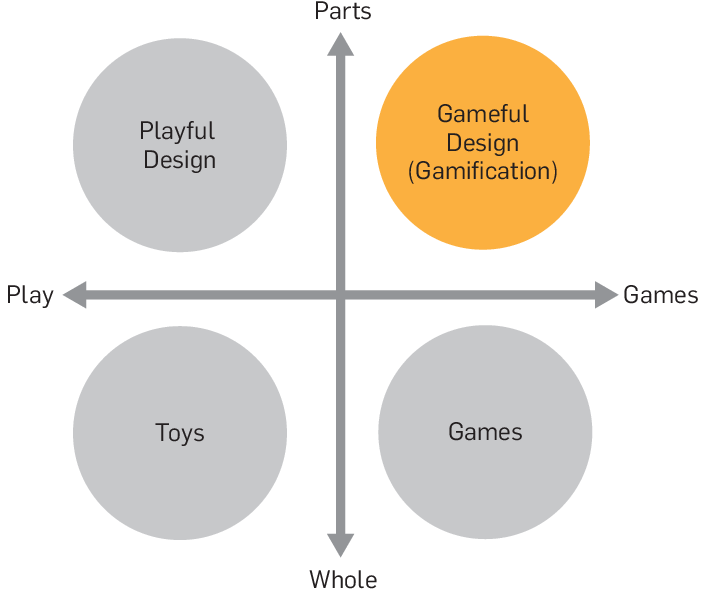
\includegraphics{img/detering_gamificatrion_pic.png}
    \caption{Abgrenzung von Gamification, Serious Games und Playful Design nach Deterding et al (2011)}
    \label{fig:deterding}
\end{figure}

Serious Games lassen sich grob in die Kategorien Educational  Games, 
Corporate  Games,  Health  Games,  Persuasive  Games,  Music  Games  sowie  Virtual  Worlds  und 
Mobile Learning Games unterteilen \cite[S.4]{bopp_serious_2009}.
Für diese Arbeit ist lediglich die Kategorie der Educational  Games relevant.
Bei dieser Art der Serious Games geht es um den pädagogischen Einsatz von Videospielen.
Charakteristisch für Educational  Games ist, dass die Lernerfahrung ein spezifisches Ziel verfolgt \cite{nielsen_overview_2006, bopp_serious_2009}.
Typischerweise besteht ein solches Ziel in der Vermittlung bestimmter Fähigkeiten, wie Algebra, Rechtschreibung und weiteren Grundfertigkeiten.
Derartige Spiele fallen auch unter den Oberbegriff Edutainment \cite{nielsen_overview_2006}.
Diese Art der Spiele bietet den Spielern befriedigende Aufgaben, die zu der Entwicklung von neuen Fähigkeiten und Strategien führt \cite{stapleton_serious_2004}.
\citeauthorwithyear{vlachopoulos_effect_2017} bestätigen die umfassende empirische Evidenz in Bezug auf kognitive Lernergebnisse einschließlich Wissenserwerb, konzeptuelle Anwendung und Inhaltsverständnis.

Obwohl es eine Vielzahl unterschiedlicher Educational Games gibt, müssen nicht zwangsläufig vollwertige Spiele entworfen werden, um einen positiven Effekt in der Lehre zu beobachten. Neben Serious Games ist der ist der Einsatz von Spielmechaniken in der Bildung ein durchaus aktives Forschungsgebiet \cite{ibanez_gamification_2014,landers_enhancing_2017}. Da der Lernerfolg wesentlich durch Motivation, Interesse und Engagement der Lernenden bedingt ist \cite{astin_student_1984}, sind Spielmechaniken ein vielversprechendes Mittel, um die Leistung der Lernenden zu erhöhen.
Dieser Bereich zählt neben Gesundheit und Fitness zu den empirisch am besten untersuchten Anwendungsgebieten in der Gamificationforschung \cite{koivisto_rise_2019}.
So wurden positive Effekte auf Motivation und Leistung mehrfach der Praxis nachgewiesen \cite{ibanez_gamification_2014,hamzah_influence_2015,strmecki_gamification_2015}. Weniger, aber dennoch tendenziell vielversprechende, Ergebnisse finden sich im Kontext der Programmierung, die thematisch viele Überschneidungen mit der Bedienung der Kommandozeile hat. So konnten \citeauthorwithyear{layth_khaleel_empirical_2019} eine Verbesserung der Lernleistung im Kontext von Programmieraufgaben feststellen. Zu ähnlichen Ergebnissen kommen \cite{ortiz_gamification_2017}. Anzumerken ist jedoch, dass Letztere zwar eine Verbesserung des Engagements feststellen konnten, allerdings keine Auswirkungen auf die Motivation ersichtlich war.



% Kurzer Text zu unterschiedlichen Spiellementen
\subsection{Spielelemente}\label{gamelelements}
Ebenso wie es unterschiedliche Definitionen für Gamification gibt, exisitieren unterschiedliche Definitionen für Spielelemente. Ein naiver Ansatz könnte sein, Spielelemente als Reihe von spielspezifischen Bausteinen und Merkmalen zu definieren. Es stellt sich jedoch die Frage, was tatsächlich spielspezifisch ist. Eine sehr strenge Auslegung dieser Definition würde z.B. eine sehr kleine Menge von Spielelementen liefern. Avatare, Abzeichen oder Ranglisten sind in der Gamification häufig verwendete Spielelemente. Gleichwohl findet sich für jedes genannte Spielelement ein völlig spielfremdes Gegenbeispiel. So werden Avatare auf Jobbörsen verwendet (LinkedIn), Abzeichen als Verdienstauszeichnung für besondere Leistungen verliehen (Bundesverdienstkreuz) und Ranglisten auf Produktvergleichsportalen verwendet (Stiftung Warentest). Eine sehr liberale Auslegung der Definition würde wiederum Elemente einschließen, bei denen es sich offensichtlich nicht um Spielelemente handelt. Als Beispiel seien hier Waffen und Gewalt genannt. Eine große Anzahl an Spielen beinhaltet die Verwendung von Waffen oder Darstellung von Gewalt. Dennoch handelt es sich dabei nicht um Spielelemente. \citeauthorwithyear{deterding_game_2011} schlagen daher vor, Gamifizierung auf die Beschreibung von Elementen zu beschränken, die für Spiele charakteristisch sind - Elemente, die in den meisten (aber nicht notwendigerweise allen) Spielen zu finden sind, die leicht mit Spielen in Verbindung gebracht werden können und eine bedeutende Rolle im Spiel spielen. Diese Autoren weisen explizit darauf hin, dass dies eine heuristische Definition, mit viel Raum für Diskussionen darüber, was "charakteristisch" für Spiele ist, ist. \citeauthorwithyear{Reeves2009Total} haben in diesem Zusammenhang zehn Spielemente identifiziert, die \qq{gelungene} Spiele ausmachen:

\begin{enumerate}
  \item Die Möglichkeit der Selbstdarstellung (Avatar)
  \item Das Vorhandensein einer räumlichen Spielwelt (3D Welt)
  \item Ein Narrativ (Eine Geschichte, die das Spiel leitet)
  \item Direktes Feedback
  \item Punktesysteme, Ranglisten und Level (Reputation)
  \item Marktplätze und Ökonomien
  \item Wettbewerbsregeln 
  \item Teams
  \item Gegenseitiger Austausch und Kommunikation unter den Spielern
  \item Zeitdruck
\end{enumerate}

Die beiden in dieser Arbeit verwendeten Spielelemente sind Abzeichen und Fortschrittsbalken. Abzeichen stellen eine Anerkennung für erbrachte Leistung dar und können damit zu den \qq{gelungenen} Spielelementen (Reputation) gezählt werden. Die Fortschrittsanzeige erlaubt Rückschlüsse auf die Gesamtdauer des Experiments und gibt zudem direktes Feedback über den eigenen Fortschritt. Beide Designelemente lassen sich außerdem vergleichsweise einfach in eine Terminalemulation integrieren, da jedes Spielelement in sich abgeschlossen (keine Abhängigkeiten von anderen Designelementen) ist. Dadurch, dass sowohl Abzeichen als auch Fortschrittsanzeige eigenständig funktionieren sollten, ist zudem eine individuelle Bewertung des jeweiligen Spielelements möglich. Dies ermöglicht die Beurteilung der tatsächlichen Wirksamkeit und Effektivität der einzelnen Spielelemente. Eine solche Einzelfallbetrachtung ist in der Wissenschaft nicht zwangsläufig gegeben. Tatsächlich weisen \citeauthorwithyear{mazarakis2018gamification} in ihrer Analyse darauf hin, dass es nahezu unmöglich ist, den tatsächlichen Beitrag einzelner Spielelemente an einer Motivationssteigerung zu messen, da diese häufig kombiniert werden. Aus diesem Grund ist es sinnvoll, einzelne Spielelemente individuell zu untersuchen.


%-------------------------------------------------------------------------------
% Abzeichen
%-------------------------------------------------------------------------------
\subsubsection{Spielelement Abzeichen}\label{badge}
Das Abzeichen ist eines der prominentesten Spielelemente und dürfte aus dem Alltag bekannt sein. Konzerne die Abzeichen in ihren Produkten einsetzen sind zum Beispiel TripAdvisor, Google, Starbucks oder GitHub. Konkret handelt es sich dabei um digitale, visuelle Artefakte, die dem Nutzer für die Erfüllung definierter Aufgaben verliehen werden \cite{antin_badges_2011}. \citeauthorwithyear{antin_badges_2011} unterteilen Abzeichen anhand ihrer sozialpsychologische Funktion in fünf Kategorien: Zielsetzung (Goal setting), Anweisung (Instruction), Reputation (Reputation),
Status/Bestätigung (Status / Affirmation) und Gruppenidentifizierung (Group Identification). 


\paragraph{Zielsetzung}
Abzeichen fordern den Nutzer dazu heraus, ein definiertes Ziel zu erreichen. Individuen streben selbst dann nach dem Erreichen bestimmter Ziele oder Meilensteine, wenn sie selber keinerlei physische Gegenleistung erfahren. Die in einem Abzeichen dargestellten Ziele sind allerdings nicht immer explizit, etwa weil die notwendigen Aktivitäten subjektiv oder unpräzise definiert sind. Aus diesen Grund ist es wichtig, den Nutzer durch regelmäßiges Feedback auf seinen aktuellen Fortschritt hinzuweisen. 

\paragraph{Anweisung}
Abzeichen können richtungweisend wirken. So geben Abzeichen einen Hinweis darauf, welche Arten von Aktivität innerhalb eines Systems möglich sind. Diese Funktion ist nützlich, um neue Benutzer in eine bestimmte Richtung zu lenken, aber auch um bestehenden Nutzern neue Wege zu offenbaren. Dabei ist es nicht notwendig, dass Nutzer die Abzeichen tatsächlich erreichen. Alleine das bloße Betrachten der verfügbaren Abzeichen gibt dem Nutzer Aufschluss über wertgeschätzte Aktivitäten.

\paragraph{Reputation}
Abzeichen blinden die Grundlage für die Reputationsbewertungen einzelner Nutzer. Durch die Kapselung von Interessen, Fachwissen und vergangener Interaktionen helfen Abzeichen bei der Beurteilung der Reputation. So geben einsehbare Abzeichen einen Einblick in nutzerspezifische Interessen, bieten einen Überblick über Fähigkeiten und Fachwissen und dienen der Einschätzung der Vertrauenswürdigkeit und der Zuverlässigkeit eines Nutzers. Zugleich zeigen geben sie einen Hinweis auf bereits erbrachte Leistungen.

\paragraph{Status/Bestätigung}
Abzeichen wirken als Statussymbol. Sie verdeutlichen die eigene Leistung und bisherige Errungenschaften ohne explizite Prahlerei.
Die Macht der Statusbelohnungen ergibt sich insbesondere aus der Erwartung, dass andere positiv auf jemanden reagieren, der durch außerordentliche Aktivitäten entsprechende Abzeichen errungen hat. Abzeichen sind auch eine persönliche Bestätigung, da sie an vergangene Errungenschaften erinnern. Sie markieren wichtige Meilensteine und sind ein Beweis für vergangene Erfolge. Sie wirken damit auf eine ähnliche Art und Weise wie klassische Trophäen oder Medaillen.

\paragraph{Gruppenidentifizierung}
Abzeichen kommunizieren eine Reihe von gemeinsamen Aktivitäten, die eine Gruppe von Benutzern anhand gemeinsamer Erfahrungen zusammenschweißen. Das Erlangen von Abzeichen kann ein Gefühl der Solidarität vermitteln und die positive Gruppenidentifikation durch die Wahrnehmung der Ähnlichkeit zwischen einem Individuum und der Gruppe erhöhen.\\

Es gibt zahlreiche wissenschaftliche Arbeiten, die die Wirksamkeit von Abzeichen analysieren. Unterschiedliche Arbeit kommen dabei zu teilweise gegensätzlichen Ergebnissen. So konnten \citeauthorwithyear{ortiz_gamification_2017} durch den Einsatz von Abzeichen zwar eine statistisch signifikante Verbesserung des Engagements der Lernenden feststellen. Allerdings war keine Verbesserung der Leistung und intrinsischen Motivation erkennbar. Gleichermaßen stellten \citeauthorwithyear{dominguez_gamifying_2013} in einem pädagogischen Kontext fest, dass Abzeichen zwar einen positiven Einfluss auf praktische Aufgaben haben, aber potentiell negativ auf schriftliche Abgaben wirken. \citeauthorwithyear{toda_dark_2018} weißt sogar explizit auf die Gefahr einer Reduzierung der Leistung, unerwünschter Seiteneffekte und potentiellem Motivationsverlust hin. Dieses Risiko gilt es den zahlreichen positiven Effekten gegenüber zu stellen. Nennenswert ist hier insbesondere das gesteigerte Engagement, welches von unterschiedlichen Autoren beobachtet werden konnte \cite{ortiz_gamification_2017, dominguez_gamifying_2013, hamari_badges_2017, hamzah_influence_2015}. Damit bleiben Abzeichen ein überaus vielversprechendes Spielelement. 


%-------------------------------------------------------------------------------
% Fortschrittsbalken
%-------------------------------------------------------------------------------
\subsubsection{Spielelement Fortschrittsbalken}\label{progressbar}
Das Spielelement Fortschrittsbalken ist ebenfalls ein etabliertes visuelles Spielelement.
Dabei handelt es sich um ein visuelles Anzeigeelement, das den aktuellen Fortschritt eines Auftrags in Form eines Balkens repräsentiert. Dabei können selbst einfachste Fortschrittsanzeigen positiv auf die Motivation der Nutzer wirken \cite{mazarakis2018gamification}. Ein klassisches Beispiel ist etwa die Darstellung des Fortschritts einer Installation oder eines Ladevorgangs. Im wesentlichen kann man Fortschrittsanzeigen in zwei Kategorien einteilen. Zum einen gibt es die bestimmte Anzeige, die den absoluten Fortschritt eines Vorgangs anzeigt. Die Anzeige gibt somit Aufschluss auf die verbleibende Restdauer des Vorgangs. Häufig verfügen bestimmte Anzeigen zusätzlich über eine Prozentangabe. Auf der anderen Seite existieren unbestimmte Fortschrittsanzeigen. Diese erlauben keinerlei Rückschluss auf den aktuellen Fortschritt. Dies kann beispielsweise durch einen Teilbalken, der sich fortwährend von links nach rechts bewegt, realisiert werden. Fortschrittsanzeigen finden sich sehr häufig in digitalen Systemen, wie etwa Computerprogrammen, oder in Umfragen. Durch den Einsatz von entsprechenden Anzeigen in Umfragen wird sich in der Regel eine höhere Abschlussquote versprochen. Diese Hoffnung bewahrheitet sich jedoch in empirischen Untersuchungen nicht \cite{Heerwegh}. So verzeichneten Umfragen mit Fortschrittsbalken geringere Abschlussquoten als Umfragen ohne Fortschrittsindikatoren \cite{liu_examining_2017}. Trotzdem bleibt auch die Fortschrittsanzeige ein vielversprechendes Spielelement. Zum einen gibt es einfach weniger Forschungsergebnisse als bei anderen Spielelementen \cite{koivisto_rise_2019} und zum Anderen gibt durchaus positive Ergebnisse. \citeauthorwithyear{olsson_visualisation_2016} kommen in ihrer Arbeit zu dem Ergebnis, dass ein Fortschrittsbalken eine geeignete Maßnahme ist, um den Überblick der Kursteilnehmer in Online-Umgebungen zu verbessern. Gleichzeitig weisen die Autoren auf einen möglichen positiven Einfluss von Abzeichen auf die Motivation der Teilnehmer hin. Dies kann durch das Gefühl der Vollendung erklärt werden, welches wiederum ein Gefühl der Zufriedenheit vermittelt \cite{ryan_deci_2000}.

\subsection{Motivationstheorie}
Es existieren unterschiedlichste Modelle, die die Wirkung von Gamification erklären. Ein weit verbreiteter Ansatz ist die Selbstbestimmungstheorie nach \citeauthorwithyear{ryan2017self}. Diese wird sehr häufig verwendet, um die Wirkung von Gamification zu erklären\cite{rapp2019strengthening}.

\subsubsection{Selbstbestimmungstheorie}
Die Selbstbestimmungstheorie (\textit{Self Determination Theory}, kurz SDT) nach \citeauthorwithyear{ryan2017self} geht davon aus, dass Menschen fleißig und mühevoll Leistung erbringen, wenn drei wesentliche psychologische Grundbedürfnisse erfüllt sind: Kompetenz (\textit{Competence}), Autonomie (\textit{Autonomy}) und Zugehörigkeit (\textit{Relatedness}).

 \paragraph{Kompetenz}
 Mit Kompetenz ist im Kern das Bedürfnis, eine Aufgabe zu meistern, gemeint. Dieses Bedürfnis ist erfüllt, wenn die Person sich fähig fühlt und das Gefühl hat, eine Aufgabe effektiv zu bewältigen \cite{ryan2017self}. Dies ist insbesondere dann der Fall, wenn das Individuum den Anforderungen gerecht wird und die eigenen Fähigkeiten als ausreichend wahrgenommen werden. Gleichwohl kann das Grundbedürfnis nach Kompetenz nicht erfüllt werden, wenn Aufgaben die eigene Fähigkeit übersteigen oder die ausführende Person ausschließlich negatives Feedback erhält. Geeignete Spielelemente, die das subjektiv wahrgenommene Gefühl der Kompetenz positiv beeinflussen, sind nach \citeauthorwithyear{sailer2016wirkung} Punkte, Leistungsgraphen oder Ranglisten. Diese Spieldesignelemente geben positives Feedback und heben die eigene Leistungsfähigkeit hervor.
 
 
 \paragraph{Autonomie}
 Unter Autonomie verstehen \citeauthorwithyear{ryan2017self} das Grundbedürfnis der Wahlfreiheit. Dieses Bedürfnis ist erfüllt, wenn das Individuum das Gefühl hat, sich freiwillig und ohne äußeren Zwang für bestimmte Tätigkeiten entscheiden zu können. Diese Tätigkeit sollten den eigenen Wertvorstellungen entsprechen und als positiv wahrgenommen werden. Zusätzlich muss die Person möglichst in der Lage sein, das eigene Handeln eigenständig zu steuern, und sich als alleiniger Herr der eigenen Entscheidungen wahrnehmen. Negativ wirken äußere Zwänge, fehlende Wahlmöglichkeiten oder fehlendes Mitspracherecht. Auch dieses Bedürfnis kann durch Spielelemente zusätzlich befriedigt werden. So erhöhen Avatare das Gefühl der Wahlfreiheit \cite{sailer2016wirkung}.
  
\paragraph{Zugehörigkeit}
Das Bedürfnis nach Zugehörigkeit und sozialer Eingebundenheit ist erfüllt, wenn sich eine Person mit anderen Personen verbunden fühlt. Diese Verbundenheit entsteht durch sozialen Kontext und durch subjektiv wahrgenommene, soziale Nähe. Fühlen sich Personen nicht in der Lage, einen Mehrwert für die Gruppe zu liefern, oder empfinden sich entsprechende Personen überhaupt nicht als Teil einer Gruppe, kann dieses Bedürfnis nicht erfüllt werden. Durch gemeinsame Teambestenlisten kann das subjektiv wahrgenommene Gefühl des konstruktiven Wettbewerbs erhöht werden \cite{sailer2016wirkung}.


Die von mir gewählten Spielelemente Abzeichen und Fortschrittsbalken sollten das Kompetenzbedürfnis befriedigen. Ein Fortschrittsbalken gibt Aufschluss über den eigenen Fortschritt und liefert damit Kompetenzfeedback - ähnlich wie ein durch \citeauthorwithyear{sailer2016wirkung} vorgeschlagenes Punktesystem. Abzeichen wirken ähnlich, indem sie bisherigen Leistungen bestätigen und gleichzeitig die eigene Leistungsfähigkeit demonstrieren \cite{antin_badges_2011}. Aufgrund der Tatsache, dass das Erlernen der Kommandozeile mit viel Frustration verbunden sein kann und damit potentiell negativ auf das Kompetenzbedürfnis wirkt, erscheinen die gewählten Spielelemente vielversprechend.

%-------------------------------------------------------------------------------
% HCI - Kommandozeile
%-------------------------------------------------------------------------------
\subsection{Kommandozeile}
Die Kommandozeile, auch Befehlszeile, CLI (Command Line Interface) oder Terminal genannt, stellt die einfachste Form der Mensch-Computer-Interaktion dar \cite{Kumar2005}. Ein solches Programm akzeptiert Textzeilen als Eingabe, welche dann kontextabhängig ausgeführt werden. Diese Aufgabe übernimmt der Befehlsinterpreter, welcher die über die Tastatur eingegebenen Befehle interpretiert und anschließend ausführt \cite{wissen_interpreter}. 
Dadurch ist es dem Nutzer möglich, externe Programme zu starten, Konfigurationsänderungen vorzunehmen oder Manipulationen des Dateisystems vorzunehmen (Erstellen, Kopieren, Löschen von Dateien und Ordnern).

Kommandozeilen haben gegenüber graphischen Oberflächen dabei einen wesentlichen Vorteil. Durch die Kombination unterschiedlicher Befehle und verschiedener Parameter ist es möglich, komplexe Arbeitsabläufe mit minimaler Interaktion abzubilden. Für den Nutzer bedeutet dies eine gesteigerte Effizienz \cite{Kumar2005}. Gleichzeitig ist die Entwicklung einer Konsolenschnittstelle mit deutlich weniger Aufwand für den Entwickler verbunden als die Entwicklung einer graphischen Oberfläche. Allerdings erfordert die Bedienung der Kommandozeile das Wissen über Befehle, möglicher Befehlsparameter und der entsprechenden Syntax für den jeweiligen Interpreter. Das Erlernen der Kommandozeile ist damit vergleichbar mit dem Erlernen einer Programmiersprache. Tatsächlich gibt es für etablierten Kommandozeilen eigene Skriptsprachen, die dem programmatischen Ausführen von Befehlen dienen (Bash, DOS, ZSH, usw.). Diese Eigenschaften führen dazu, dass Kommandozeilen insbesondere im professionellen Umfeld eingesetzt werden. Neben dem Einsatz in der Softwareentwicklung und Systemadministration finden sich Kommandozeilen in vielen Programmen, die auch über eine graphische Oberfläche verfügen. So verfügen AutoCAD, Adobe Photoshop, SAP und die Microsoft Office-Produkte über zusätzliche Interaktionsmöglichkeiten per Kommandozeile.



%-------------------------------------------------------------------------------
% Fragestellung
%-------------------------------------------------------------------------------

\subsection{Fragestellung und Zielsetzung}
Das Erlernen der Kommandozeile gleicht in Teilen dem Erlernen einer Programmiersprache und kann anfänglich mit einem hohen Maß an Frustration verbunden sein. Daher bietet es sich an, den Lernprozess motivierender zu gestalten, um den Lernerfolg zu erhöhen. Daher ist es wenig verwunderlich, dass es unzählige unterschiedliche im weitesten Sinne \qq{gamifizierte} Konsolenanwendungen im Internet gibt. Dabei handelt es sich häufig um interaktive Text-Adventures. Drei auffallend liebevoll gestaltete Beispiele hierfür sind LostKingdom\footnote{Link: https://rdebath.github.io/LostKingdom/}, TheLab\footnote{Link: https://gfc.albertocongiu.com/thelab/}und Adventex\footnote{Link: https://thoster.net/adventex/}. Die Wirksamkeit entsprechender Anwendungen wurde bisher jedoch nie empirisch untersucht. 

Im Rahmen der Arbeit werden daher die Spielelemente Abzeichen und Fortschrittsbalken in eine Webanwendung integriert, die der Vermittlung grundlegender Kommandozeilenbefehlen dient. Anschließend wird der Einfluss der Spielelemente hinsichtlich Motivation und Leistung der Benutzer untersucht. Wie in Abschnitt \ref{gamelelements} geschildert, zeigen beide Spielelemente positive Effekte auf die Lernleistung von Lernenden und sind daher vielversprechende Designelemente. Die zugrundeliegende Forschungsfrage lautet daher:

\begin{itemize}
    \item Welchen Einfluss haben die Spieldesignelemente Abzeichen und Fortschrittsbalken auf Motivation und Leistung im Kontext der Kommandozeile?
\end{itemize}

Daraus leiten sich die folgenden Hypothesen ab:

\begin{itemize}
\item H1: Probanden, die Abzeichen erhalten, beantworten im Mittel eine höhere Anzahl an Fragen als eine Kontrollgruppe ohne Abzeichen.
\item H2: Probanden, die eine Fortschrittsanzeige sehen, beantworten im Mittel eine höhere Anzahl an Fragen als eine Kontrollgruppe ohne Fortschrittsanzeige.
\end{itemize}

Die Ergebnisse sind für alle Personen interessant, die Berührungspunkte mit der Kommandozeile haben.
Hervorzuheben sind insbesondere Schüler und Studenten, die keinerlei bestehende Erfahrung mit einer rein textbasierten Nutzerschnittstelle haben. Die entstehende Anwendung könnte zukünftig dazu dienen, Einsteigern bei dem Erlernen der Kommandozeile zu unterstützen. Gleichzeitig liefert die Arbeit weitere empirische Daten hinsichtlich der Wirkung von Abzeichen und Fortschrittsanzeige.